\section{Interactive User Interface}
\subsection{Process}
\begin{enumerate}
    \item{The user makes a request to the frontend by visiting the website in their browser.}
    \item{The frontend router handles the request and displays the page requested.}
    \item{The user sends a message by typing into the text field on the chat page.}
    \item{The frontend detects that the user is awaiting a response and displays a loading animation.}
    \item{The message is stored in an internal \code{Vuex} state and is also sent to the backend via a lazily created websocket.}
    \item{The backend sends a response back to the frontend through the same websocket.}
    \item{The response is stored in the \code{Vuex} state.}
    \item{The frontend detects a change and renders the page again to end the loading animation and display the response.}
\end{enumerate}

\subsection{Example Usage}
This is an example use case based on the first user story described in section 2.1.1.

The student visits the homepage for the chat bot and is greeted by the welcome screen. They are then able to register by inputting a username, which can be anything from their real name to their zID. There is no other information required for registration to make it fast and easy to use. Password authentication was deemed not required, as no sensitive data can be accessed.

\begin{center}
    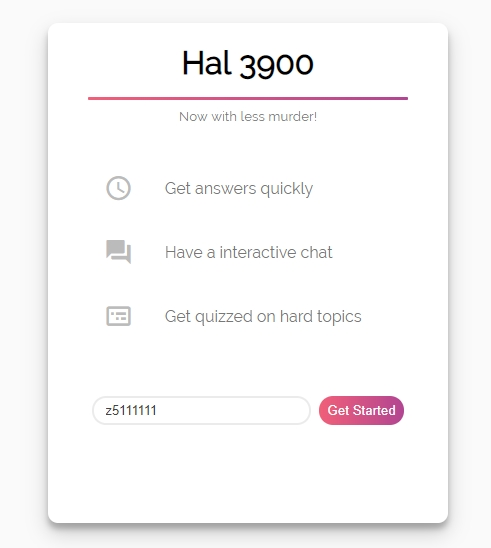
\includegraphics[width=7cm]{register.jpg}
\end{center}

Once logged in, the user can use the intuitive chat interface to interact with the chat bot. They are free to ask questions about anything relevant, including the course content or for a quiz. In this case, the student would like to learn more about the course administration.

\includegraphics[width=\textwidth]{chat-log.png}

\subsection{Technical Details}
The web interface is developed using \code{Vue.js}. This allows us to build a modular and extensible frontend with reusable components. For example, the generic message base component was extended to allow the bot to respond with a number of message formats, such as a regular message, a set of options that can be selected from, a quiz question and answer pair, or a table.

\code{Vuex} is a state management pattern and library that was used to centralise the data that the frontend needs to access. This helps to limit the number of times the page needs to be rendered after a change is made. It also allows for complex logic, such as expressing the chat bot as a set of components. Implementing this helped us add features in short sprint cycles as it eliminated the need to constantly move around large amounts of information.

\code{TypeScript} was also used here for reasons similar to those described in other facets of our system. It helps mitigate the problems that come with \code{JavaScript} such as undefined or malformed variables, allowing us to avoid or handle errors better.

We also used \code{Sass} to quickly and cleanly style our website. This was done to make the user interface as pleasant and usable as possible for the end user.

\newpage
